\documentclass[11pt]{article}
\usepackage[margin=1in]{geometry}
\usepackage{amsmath,amsthm,amssymb}
\usepackage{enumitem, graphicx, float, caption}
\usepackage{amsmath}
\usepackage{bm}
\usepackage{parskip}
\usepackage{lipsum}
\usepackage{tikz}
\usepackage{listings}
\usepackage{xcolor}
\usepackage{float}
\usepackage{subcaption}
\usepackage{graphicx}
\usepackage[utf8]{inputenc}
\usetikzlibrary{arrows.meta}

\definecolor{codegreen}{rgb}{0,0.6,0}
\definecolor{codegray}{rgb}{0.5,0.5,0.5}
\definecolor{codepurple}{rgb}{0.58,0,0.82}
\definecolor{backcolour}{rgb}{0.95,0.95,0.92}

\lstdefinestyle{mystyle}{
    backgroundcolor=\color{backcolour},
    commentstyle=\color{codegreen},
    keywordstyle=\color{magenta},
    numberstyle=\tiny\color{codegray},
    stringstyle=\color{codepurple},
    basicstyle=\ttfamily\tiny,
    breakatwhitespace=false,
    breaklines=true,
    captionpos=b,
    keepspaces=true,
    numbers=left,
    numbersep=5pt,
    showspaces=false,
    showstringspaces=false,
    showtabs=false,
    tabsize=2
}

\makeatletter
\renewcommand*\env@matrix[1][\arraystretch]{%
  \edef\arraystretch{#1}%
  \hskip -\arraycolsep
  \let\@ifnextchar\new@ifnextchar
  \array{*\c@MaxMatrixCols c}}
\makeatother

\lstset{xleftmargin=.020\textwidth, xrightmargin=.020\textwidth}

\setcounter{MaxMatrixCols}{26}
\setlength\parindent{0pt}
\counterwithin{equation}{enumi}


\begin{document}
    \noindent Nathan Burwig \\
    Math 87 HW 8 \\
    Due My Birthday :)
    
    \hrulefill
    
    \section{Spline Interpolation}
    
    Manually form a matrix for cubic spline interpolation of f(x) with natural 
    and with clamped boundary conditions, if
    \[
        f(0) = 0,\; f(1) = 2,\; f(2) = 1
    \]
    You may use numpy to solve the resulting linear systems for coefficients.

    \begin{enumerate}
        \item In order to complete cubic spline interpolation there are several
            factors we will want to take into account. The first, are the
            conditions in place from our data points. Those are the points
            listed above. We can list the constraints they impart on our system
            as follows...
            \begin{alignat}{3}
                f_1(0) \;&=\; x^3a_1 + x^2b_1 + xc_1 + d_1 \;&&=\; d_1 & &= 0  \\
                f_1(1) \;&=\; x^3a_1 + x^2b_1 + xc_1 + d_1 \;&&=\; a_1 + b_1 + c_1 + d_1 & &= 2 \\
                f_2(1) \;&=\; x^3a_2 + x^2b_2 + xc_2 + d_2 \;&&=\; a_2 + b_2 + c_2 + d_2 & &= 2 \\
                f_2(2) \;&=\; x^3a_2 + x^2b_2 + xc_2 + d_2 \;&&=\; 8a_2 + 4b_2 + 2c_2 + d_2 & &= 1 
            \end{alignat}
            Along with these constraints, we also require that our system is
            continuous at both points, which means both the first and second
            derivatives must be equal to eachother at those points. The
            constraints for the first derivative are as follows...
            \[
                \frac{df_1(x)}{dx} = \frac{df_2(x)}{dx}
            \]
            Which implies..
            \begin{equation}
                0 = 3a_1 + 2b_1 + c_1 - 3a_2 - 2b_2 - c_2  
            \end{equation}
            And the constraint on the second derivative we get...
            \[
                \frac{d^2f_1(x)}{dx^2} = \frac{d^2f_2(x)}{dx^2} 
            \]
            Which further implies...
            \begin{equation}
                0 = 6a_1 + 2b_1 - 6a_2 - 2b_2
            \end{equation}
            We now turn to the final condition we express, which are the
            boundary constraints. These are either natural or clamped, and will
            have an impact in our final matrix. The \textit{natural} constraint dictates
            that the second derivatives of the end points must be equal to
            zero. The \textit{clamped} constriants dicate that the first
            derivatives must be equal to zero at the endpoints.

            Natural:
            \begin{alignat}{3}
                f^{''}_1(x_0) \;&=\; 6a_1x + 2b_1 \;&&=\; 2b_1 & &= 0 \\
                f^{''}_2(x_n) \;&=\; 6a_2x + 2b_2 \;&&=\; 2a_2 + 2b_2 & &= 0
            \end{alignat}
            Clamped:
            \begin{alignat}{3}
                f^{'}_1(x_0) \;&=\; 3a_1x^2 + 2b_1x + c_1 \;&&=\; c_1 & &= 0 \\
                f^{'}_2(x_n) \;&=\; 3a_2x^2 + 2b_2x + c_2 \;&&=\; 12a_2 + 4b_2 + c_2& &= 0
            \end{alignat}
            Now that we have our boundary conditions setup, we can setup two
            different linear systems of these equations, one with the natural
            condition and one with the clamped. Then we can solve these systems
            for the coefficients of the cubic polynomials which satisfy all the
            constraints we've given.

            Natural:
            \[
                \left[
                \begin{array}{cccccccc}
                    0 & 0 & 0 & 1 & 0 & 0 & 0 & 0   \\
                    1 & 1 & 1 & 1 & 0 & 0 & 0 & 0   \\
                    0 & 0 & 0 & 0 & 1 & 1 & 1 & 1   \\
                    0 & 0 & 0 & 0 & 8 & 4 & 2 & 1   \\
                    \hline  
                    3 & 2 & 1 & 0 &-3 &-2 &-1 & 0   \\
                    \hline
                    6 & 2 & 0 & 0 & 0 & 0 & 0 & 0   \\
                    \hline
                    0 & 2 & 0 & 0 & 0 & 0 & 0 & 0   \\
                    0 & 0 & 0 & 0 & 6 & 2 & 0 & 0   
                \end{array}
                \right]
                \begin{bmatrix}
                    a_1 \\ b_1 \\ c_1 \\ d_1 \\ a_2 \\ b_2 \\ c_2 \\ d_2
                \end{bmatrix}
                =
                \begin{bmatrix}
                    0 \\ 2 \\ 2 \\ 1 \\ 0 \\ 0 \\ 0 \\ 0 
                \end{bmatrix}
            \]
            I have delineated the different constraints being used by the
            horizontal lines. The first four are associated with constraints
            1.1-4, then 1.5, 1.6 and 1.7-8.

            Clamped:
            \[
                \left[
                \begin{array}{cccccccc}
                    0 & 0 & 0 & 1 & 0 & 0 & 0 & 0   \\
                    1 & 1 & 1 & 1 & 0 & 0 & 0 & 0   \\
                    0 & 0 & 0 & 0 & 1 & 1 & 1 & 1   \\
                    0 & 0 & 0 & 0 & 8 & 4 & 2 & 1   \\
                    \hline  
                    3 & 2 & 1 & 0 &-3 &-2 &-1 & 0   \\
                    \hline
                    6 & 2 & 0 & 0 & 0 & 0 & 0 & 0   \\
                    \hline
                    0 & 0 & 1 & 0 & 0 & 0 & 0 & 0   \\
                    0 & 0 & 0 & 0 &12 & 4 & 1 & 0   
                \end{array}
                \right]
                \begin{bmatrix}
                    a_1 \\ b_1 \\ c_1 \\ d_1 \\ a_2 \\ b_2 \\ c_2 \\ d_2
                \end{bmatrix}
                =
                \begin{bmatrix}
                    0 \\ 2 \\ 2 \\ 1 \\ 0 \\ 0 \\ 0 \\ 0 
                \end{bmatrix}
            \]

            Now we can solve these quickly using the \texttt{numpy.linalg.solve()}
            function in \texttt{python}. Doing so gives us two coefficient
            vectors. Below you will see the two plots given, along with the
            associated polynomials given for the two different boundary
            conditions. 

            \begin{minipage}[t]{0.42\linewidth}
                {\footnotesize
                    Natural:
                }\\
                \begin{center}
                    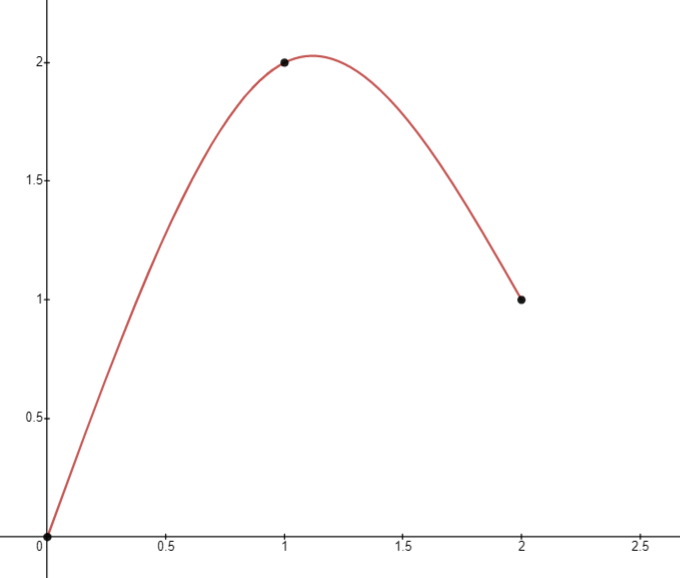
\includegraphics[width=.8\linewidth]{natural.png}
                \end{center}
                {\footnotesize
                    \begin{alignat*}{2}
                        f_1(x) &= -3.25x^3 + 5.25x^2 \;\;\; &&\left[ 0 \leq x \leq 1 \right] \\
                        f_2(x) &= 2.75x^3 - 12.75x^2 + 18x -6 \;\;\; &&\left[ 1 \leq x \leq 2 \right]
                    \end{alignat*}
                }
            \end{minipage} \hfill\vline\hfill %
            \begin{minipage}[t]{0.42\linewidth}
                {\footnotesize
                    Clamped
                }\\
                \begin{center}
                    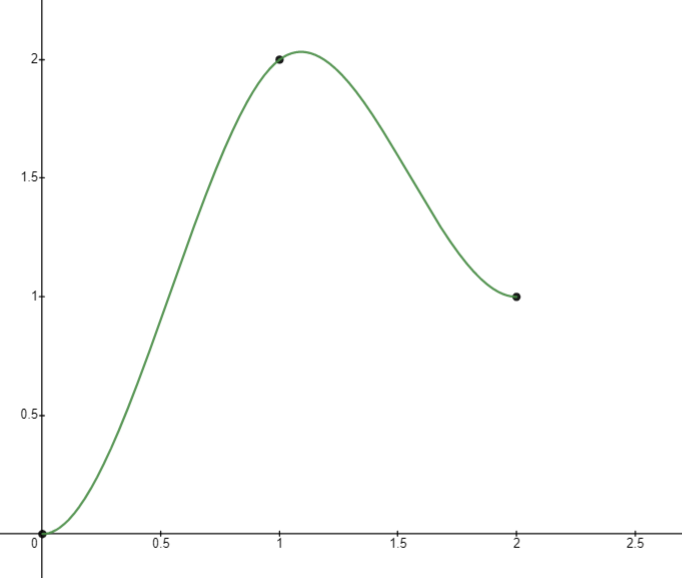
\includegraphics[width=.8\linewidth]{clamped.png}
                \end{center}
                {\footnotesize
                    \begin{alignat*}{2}
                        f_1(x) &= -3.25x^3 + 5.25x^2 \;\;\; &&\left[ 0 \leq x \leq 1 \right] \\
                        f_2(x) &= 2.75x^3 - 12.75x^2 + 18x -6 \;\;\; &&\left[ 1 \leq x \leq 2 \right]
                    \end{alignat*}
                } 
            \end{minipage} 
    \end{enumerate}

    \section{Comprehending SVM}
    Suppose we have data drawn from two different populations, shown in the 
    figure below as (+) and (--). Support vector machines could be simply used 
    to linearly separate such classes of data.
    \begin{center}
        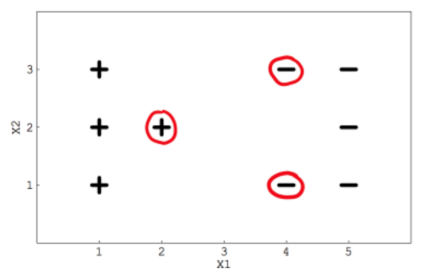
\includegraphics[width=0.6\linewidth]{og.png}
    \end{center}
    \begin{enumerate}
        \item \textbf{Draw your approximation of the separating line SVM would 
            generate to separate these two classes of data}

            We know that SVM cares about the perpendicular distance between
            nearby points on the plot. The average then would form a line that
            looks as follows.
            \begin{center}
                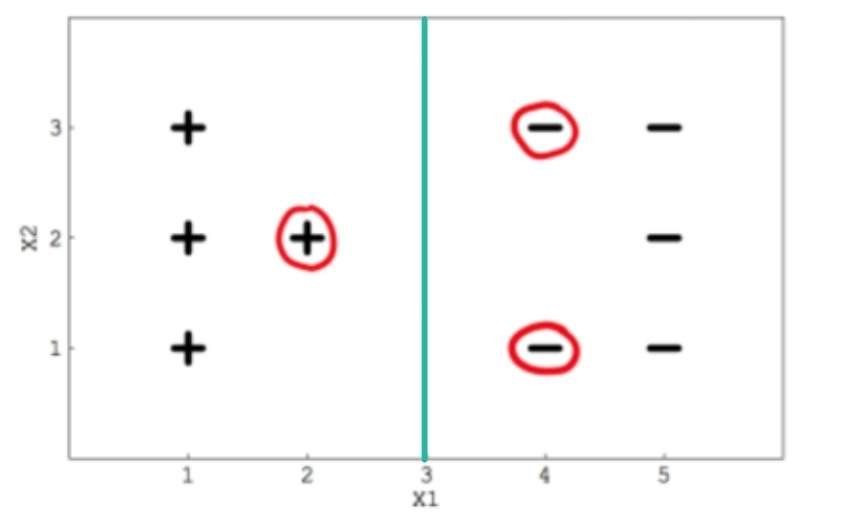
\includegraphics[width=0.5\linewidth]{first.png}    
            \end{center}
        \item \textbf{Suppose that the (+) in the red circle was deleted from 
            the data set. Would the supporting line change? If so, draw it.}

            If the plus disappears, it moves our line as follows...
            \begin{center}
                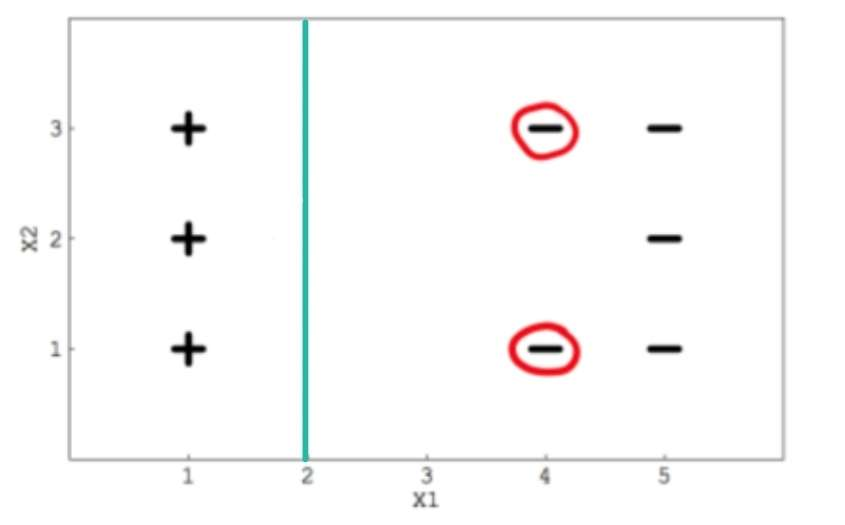
\includegraphics[width=0.5\linewidth]{second.png}    
            \end{center}
            My line being at 2 is perhaps a bit misleading, looking at it now
            it should probably be closer to 2.5 or so.
        \item \textbf{Suppose that all red circled data points were deleted. 
            Would the supporting line change? If so, draw it}

            Removing all red points would move the line as follows...
            \begin{center}
                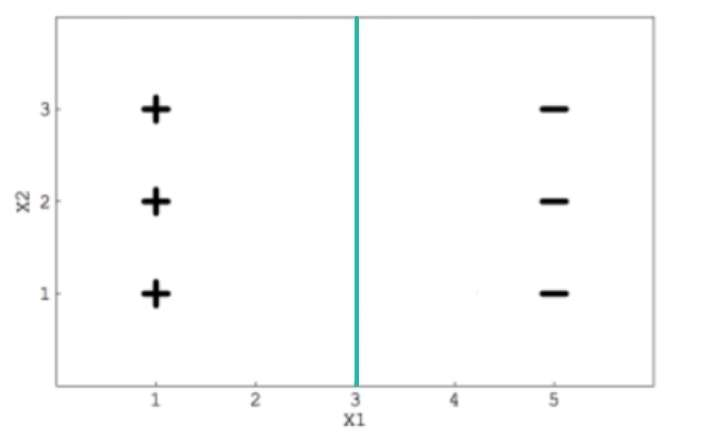
\includegraphics[width=0.5\linewidth]{last.png}    
            \end{center}
    \end{enumerate}
    \newpage

    \section{Computing Kernels}
    Let $\hat{x} = \langle x_1, x_2 \rangle$ and $\hat{y} = \langle y_1, y_2 \rangle$ 
    both $\in \mathbb{R}^2$. Suppose we use the kernel function
    $K(\hat{x},\hat{y})=(\hat{x} \cdot \hat{y} + c)^2$. Compute the higher
    dimensional embedding (i.e. the feature map) of $\hat{x}$ corresponding to
    this kernel.

    \begin{enumerate}
        \item   We would like to determine the higher dimensional embedding
            imposed by the kernel given above. We know that the dimensionality
            will be {\footnotesize $\left( \begin{array}{c} n + d \\ d \end{array} \right)$} 
            Where $n$ is the original dimension of the 
            problem, and $d$ is the power to which we are raising our kernel. 
            So, we expect this projection to go into $\mathbb{R}^6$

            We can start by just expanding out the inner product we have in our
            kernel function.
            \begin{align*}
                K(\hat{x},\hat{y}) &= (\hat{x} \cdot \hat{y} + c)^2 \\
                             &= (x_1y_1 + x_2y_2 + c)^2 \\
                             &= ((x_1y_1)^2 + (x_2y_2)^2 + 2x_1x_2y_1y_2 + 2cx_1y_1 + 2cx_2y_2 + c^2 \\
            \end{align*}
            It is here we can note that this whole expression can be written
            out in terms of a rather long winded dot product. They can be
            arranged in a couple of different orders, but in general I will
            separate the $x$'s from the $y$'s.
            \[
                \begin{bmatrix}[1.3]
                    x_1^2   \\
                    x_2^2   \\
                    \sqrt{2}x_1x_2  \\
                    \sqrt{2c}x_2    \\
                    \sqrt{2c}x_1    \\
                    c
                \end{bmatrix}^T
                \begin{bmatrix}[1.3]
                    y_1^2   \\
                    y_2^2   \\
                    \sqrt{2}y_1y_2  \\
                    \sqrt{2c}y_2    \\
                    \sqrt{2c}y_1    \\
                    c
                \end{bmatrix}
            \]            
            We can manually multiply this out and we see...
            \[
                (x_1y_1)^2 + (x_2y_2)^2 + 2x_1x_2y_1y_2 + 2cx_2y_2 + 2cx_1y_1 + c^2
            \]
            Which is exactly what we started with. Thus we can define the
            higher dimensional embedding from our kernel as the following
            feature map.
            \[
                \phi(x) = \begin{bmatrix}[1.3]
                            x_1^2   \\
                            x_2^2   \\
                            \sqrt{2}x_1x_2  \\
                            \sqrt{2c}x_2    \\
                            \sqrt{2c}x_1    \\
                            c
                       \end{bmatrix}
            \]
    \end{enumerate}
\end{document}

